\documentclass[10pt,a4paper]{article}
\usepackage[utf8]{inputenc}
\usepackage[english]{babel}
\usepackage[left=2cm,right=2cm,top=2cm,bottom=2cm]{geometry}
\usepackage{amsmath}
\usepackage{amsfonts}
\usepackage{amssymb}
\usepackage{graphicx}
\usepackage{fourier}
\usepackage{listings}
\usepackage{biblatex}
\usepackage{minted}
\usepackage{csquotes}
\usepackage{hyperref}
\usepackage{caption}
\usepackage{subcaption}
\addbibresource{ref.bib}
\title{A Genetic Algorithm for the Traveling Salesman Problem}
\author{Francisco J. Palmero Moya}
\begin{document}
\maketitle
\begin{abstract}
    The present document shows a Genetic Algorithm approach for the Traveling Salesman Problem. The study primarily investigates the interplay between crossover probability and the effectiveness (including efficiency) of the genetic algorithm. It delves into how the crossover probability influences the quality and convergence speed of results, demonstrated through instances of varying complexities in the Traveling Salesman Problem.
\end{abstract}
\section{Introduction}
Evolutionary Computing (EC) is a research area within computer science, which draws inspiration from the process of natural evolution. In essence, we can consider natural evolution as follows: a given environment is filled with a population of individuals that strive for survival and reproduction. The fitness of these individuals is determined by the environment, and relates to how well they succeed in achieving their goals. Similarly, in EC, a population of potential solutions to a problem evolves over successive generations through mechanisms such as selection, crossover, and mutation, ultimately converging towards optimal or near-optimal solutions in complex optimization and search tasks. 

The algorithms involved in EC are termed Evolutionary Algorithms (EAs). The common underlying idea behind all these techniques is the same: given a population of individuals within some environment that has limited resources, competing for those resources causes natural selection. Given a quality function to be maximised, we can randomly create a set of candidates solutions. We then apply the quality function to these as an abstract fitness measure, and some of the better candidates are chosen to seed the next generation. This is done by applying recombination and/or mutation to them.
\begin{description}
    \item[Recombination] Recombination is an operator that is applied to two or more selected candidates (the so-called parents), producing one or more new candidates (the children).
    \item[Mutation] Mutation is applied to one candidate and results in a new candidate slightly different.
\end{description}
Therefore executing the operations of recombination and mutation on the parents leads to the creation of a set of new candidates (the offspring). These have their fitness evaluated and then compete with the old ones for a place in the next generation. This process can be iterated until a candidate with sufficient quality is found.

There are two main forces that form the basis of evolutionary systems:
\begin{enumerate}
    \item Variation operators (recombination and mutation) create the necessary diversity within the population, and thereby facilitate novelty.
    \item Selection acts as a force increasing the mean quality of solutions in the population.
\end{enumerate}
The combined application of variation and selection generally leads to improving fitness values in consecutive populations. The general scheme of an EA is given by the pseudocode of Figure \ref{fig:EAscheme}. The main components of any EA are
\begin{itemize}
    \item representation (definition of individuals)
    \item evaluation function (or fitness function)
    \item population
    \item parent selection mechanism 
    \item variation operators, recombination and mutation
    \item survivor selection mechanism (replacement)
\end{itemize}
To create a complete, runnable algorithm, it is necessary to specify each component and to define the initialization procedure. If we wish the algorithm to stop at some stage, we must also provide a termination condition.
\begin{figure}[h!]
    \centering
    \begin{lstlisting}
        BEGIN
            INITIALISE population with random candidate solutions;
            EVALUATE each candidate;
            REPEAT UNTIL ( TERMINATION CONDITION is satisfied ) DO
                1  SELECT parents;
                2  RECOMBINE pairs of parents;
                3  MUTATE the resulting offspring;
                4  EVALUATE new candidates;
                5  SELECT individuals for the next generation;
            OD 
        END
    \end{lstlisting}
    \label{fig:EAscheme}
\caption{The general scheme of an evolutionary algorithm in pseudocode}
\end{figure}

EAs are an stochastic trial-and-error style problem solving process where performance measures are statistical in nature, meaning that a number of experiments need to be conducted to gain sufficient experimental data. The three basic performance measures are:
\begin{itemize}
    \item success rate 
    \item effectiveness (solution quality)
    \item efficiency (speed)
\end{itemize}
The study of two of them, effectiveness and efficiency, serves as a metric for the interplay between crossover probability and the effectiveness (including efficiency) of the genetic algorithm we have developed.

\section{Traveling Salesman Problem}
The Travelling Salesman Problem (TSP) is a well-known problem in computer science and operations research. It involves finding the shortest possible route that visits a given set of cities and returns to the starting city. This problem is NP-hard, meaning that it is very difficult to solve exactly, especially as the number of cities increases. 

It is believed to have originated in the early 1800s, when the Irish mathematician W.R. Hamilton posed the problem of finding a way to visit each of the 13 Irish counties and return to the starting point in the shortest possible time. This problem was later generalized to finding the shortest route between a given set of cities.

The TSP can also be conceptualized as finding a Hamiltonian path within a complete graph. In this context, the cities are represented as nodes, and the distances between them as edges. The objective is to discover a path that visits each city exactly once and returns to the starting city while minimizing the total distance traveled. This Hamiltonian path formulation encapsulates the essence of TSP by emphasizing the efficient walk to all cities while adhering to the constraint of visiting each city only once. Despite its seemingly straightforward description, the computational complexity of finding the optimal Hamiltonian path grows exponentially with the number of cities, contributing to the NP-hard nature of the TSP.

One possible approach to solving the TSP is to use a Genetic Algorithm (GA). This involves representing the route as a string of numbers, with each number representing a city in the given set. The algorithm then uses principles of natural selection to evolve the string over many iterations, with the goal of finding the shortest possible route. This is done by evaluating the fitness of each string, which corresponds to the length of the route it represents. Strings with shorter routes are more likely to be selected for reproduction, and the resulting offspring strings are mutated to introduce new variations. Over time, the algorithm converges on a high-quality solution.

\section{Methods}
The proposed GA is based on the same fundamentals ideas of EC presented in the introduction. The concrete methodology is described along this section. The GA is a possible approach to the TSP, therefore the starting point of the study is a description of how the GA address the problem. 

\paragraph*{Representation}
The cities are given by a pair of coordinates representing their position in a 2-dimensional space and its identifying name\footnote{A simple index or label is sufficient.}. The solution to the problem at hand is a Hamiltonian path where the nodes are the cities. Therefore, to set up a bridge between the original problem context and the problem-solving space where evolution takes place, one has to decide how possible solutions should be specified and stored in a way that can be manipulated by a computer. We say that objects forming possible solutions within the original problem context are referred to as phenotypes, while their encoding, are called genotypes. This firs step is commonly called representation and in TSP context should reflect the encoding of the path in the graph. It seems reasonable to use a permutation representation because its ability to solve problems where the solution is deciding on the order in which a sequence of events should occur. In the TSP, labelling the cities $1, 2, ..., N$, a complete tour is a permutation, so that for $n=4$, the routes $\left[1, 2, 3, 4 \right]$ and $\left[3, 4, 3, 2 \right]$ are both valid.

\paragraph*{Evaluation function} 
The role of the evaluation function is to represent the requirements the population should adapt to meet. The valuation function is also called the fitness function, and here we use both equally. In the TSP, the fitness function is the total path distance of a given permutation, i.e., it is the objective function we aim to optimize. It is a measure of the quality of our solution.

To achive a better performance, we compute the Euclidean Distance Matrix (EDM) before running the GA and then consult its values when the distance between cities is required. If there are $N$ cities, the EDM is a $N \times N$ symmetric matrix where the input $M_{i,j}$ represents the distance between the $i$-th and the $j$-th city.

\paragraph*{Population}
The role of the population is to hold the representation of possible solutions. A population is a multiset\footnote{A multiset is a set where multiple copies of an element are possible.} of genotypes. Although it is possible to find a heuristic for initialising the population, the proposed GA initialises the population at random by shuffling the individuals.

\paragraph*{Parent selection}
The role of parent selection is to distinguish among individuals based on their quality, and to allow the better individuals to become parents of the next generation. An individual is a parent if it has been selected to undergo variation in order to create offspring. The parent selection is performed under the tournament selection method. 

Tournament selection is an operator with the useful property that it only relies on an ordering relation that can compare and rank any two individuals. The application of tournament selection to select $\lambda$ members of a pool of $\mu$ individuals works according to the procedure shown in Figure \ref{fig:tournament}.
\begin{figure}[h!]
    \centering
    \begin{lstlisting}[escapeinside={(*}{*)}]
        BEGIN
        % Assume we wish to select (*$ \lambda $*) members of a pool of (*$ \mu $*) individuals
            set current_member = 1:
            WHILE (current_member (*$\leq \lambda$ *)) DO
                Pick (*$ k $*) individuals randomly, with or without replacement;
                Compare these (*$ k $*) individuals and select the best of them;
                Denote this individual as i;
                set mating_pool[current_member] = i;
                set current_menber = current_member + 1;
            OD 
        END
    \end{lstlisting}
    \label{fig:tournament}
\caption{The general scheme of an evolutionary algorithm in pseudocode}
\end{figure}

The tournament size $k$ is the number of individuals picked to compare them. The larger the tournament, the greater the chance that it will contain members of abive-average fitness, and the less that it will consist enterely of low-fitness members. The proposed GA set the tournament size at two and the individuals are picked at random with replacement.

\paragraph*{Variation operators}
The role of variation operators (mutation and recombination) is to create new individuals from old ones. In the corresponding phonotype space this amounts to generating new candidate solutions. A binary variation operator is called recombination or crossover. As the name indicate, such an operator merges information from two parent genotype into one or two offspring genotype. The chose crossover is a Partially Mapped Crossover (PMX) with a crossover rate $p_c$. The crossover rate is the probability of applying the PMX operator. The PMX operator is one of the most widely used operators for adjacency-type problems such as TSP. Over the years many slight variations of PMX appeared in the literature; here we followed the definition from \textcite{IntroEvComp}.

On the other hand, a unary variation is commonly called mutation. It is applied to one genotype and delivers a slighly modified mutant, the offspring. A mutation operator is always stochastic: its output depends on the outcomes of a series of random choices. Mutation operators are usually applied probabilistically according to a mutation rate $p_m$. The selected mutation is known as Swap Mutation. Two positions (genes) in the chromosome are selected at random and their allele values swapped. It can be understood as a sawp between two cities in the phenotype space.

\paragraph*{Survivor selection}
Similar to parent selection, the role of survivor selection is to distinguish among individuals based on their quality. However, it is used in a different stage of the evolutionary cycle. The survivor selection mechanism is called after the creation of the offspring from the selected parents. The proposed GA applies a generational model with elitism. The generational model implies that the current population is replaced completely by the offspring. If the elitism is applied, the current fittest member is kept in the population. Thus if it is chosen in the group to be replaced, and none of the offspring being inserted into the offspring has equal or better fitness, then it is kept and one of the offspring is discarted (in our implementation at random).

\paragraph*{Termination condition}
The GA implement the previous methods for each iteration searching the fittest individual that represent our problem solution. If the problem has a known optimal fitness level, then our termination condition would be the discovery of a solution with this fitness (given a margin error). However, EAs are stochastic and mostly there are no guarantees of reaching such an optimun, so this condition might never get satisfied, and the algorithm may never stop. Therefore we extend this condition setting a maximum number of operations.

\subsection{Implementation}
The code\footnote{The code is available at \url{https://github.com/franciscopalmeromoya/TravellingSalesmanProblem/}} designed for this problem is developed from scratch. It is written in Python and make use of common libraries of the language such as \textit{numpy, scipy, matplotlib}, etc. The code structure is divided into two main package, one for the GA and other for usuful functions for the specific problem.

The \mintinline{python}{GeneticAlgorithm} package is based on \mintinline{python}{class GeneticAlgorithm}, a Python class which handles the main functions of any GA. However, since it is developed for a concrete problem, namely the TSP, the current implemented function are specific for the problem at hand. The main advantage of the code design is its modular approach, making possible to reuse the code recoursively. If one want to use a different operator, it only requires the development of the new operator, and then insert it into the code.

Other useful functions specific for the TSP are developed into the \mintinline{python}{tools} package. There, we can find plot functions for the path and cities representation into a 2-dimensional plane or functions to load the cities coordinates from a file.

\section{Results}
The experimental evaluation is based on synthetic and existing datasets\footnote{\url{https://people.sc.fsu.edu/~jburkardt/datasets/tsp/tsp.html}}. The followed approach is different for each situation. The main parameter of our study is the crossover rate $p_c$ in all the experiments.

The two datasets used have a known optimal solution. They are of different complexity, the simples one has 16 cities and the complex one 48. These are used to study metrics such as the success rate (SR) because of the known optimal solution. They are also helpful to calibrate the model parameters, or to check if the parameters recommended by the literature work in our case.

The synthetic data is used to study other kind of metrics such as the mean best fitness, diversity, etc. Assesing the quality of an EA commonly implies experimental comparison between the given EA and other traditional algorithm. Thus, the results are compared to an heuristic path fould by linking each city to the closest one. This heuristic result can be interpreted as an anchor to compare possible solutions to the problem because it is deterministic. The SR in such context can be defined as the percentage of runs where the fitness is better than the fitness of the heuristic path.

\subsection*{Real-world datasets}
The simple problem with 16 cities have been evaluated twice: first time the crossover rate has been fixed to 0.9 and the mutation rate change between 0.5, 0.7, and 0.9; second time, mutation rate have been fixed to 0.9 (best results in first evaluation) and crossover rate change between 0.5, 0.7, and 0.9. There are 50 instances for each parameter configuration, resulting in 300 overall were the population have been kept constant at 10. The stopping criteria are a maximum number of iterations equals to 3000 or when the optimal value of 281 plus a margin of 10 is reached. The results are shown in Figure \ref{fig:mbfvsbf16}. The dashed line represents the angle bisector that divide the plane into two parts. Those points closest to the bisector and outside the success region (in green) have a MBF similar to its best fitness, meaning that the algorithm got stuck in a local minimum. Points inside the success region are spread along MBF axis. 

\begin{figure}[h!]
    \centering
    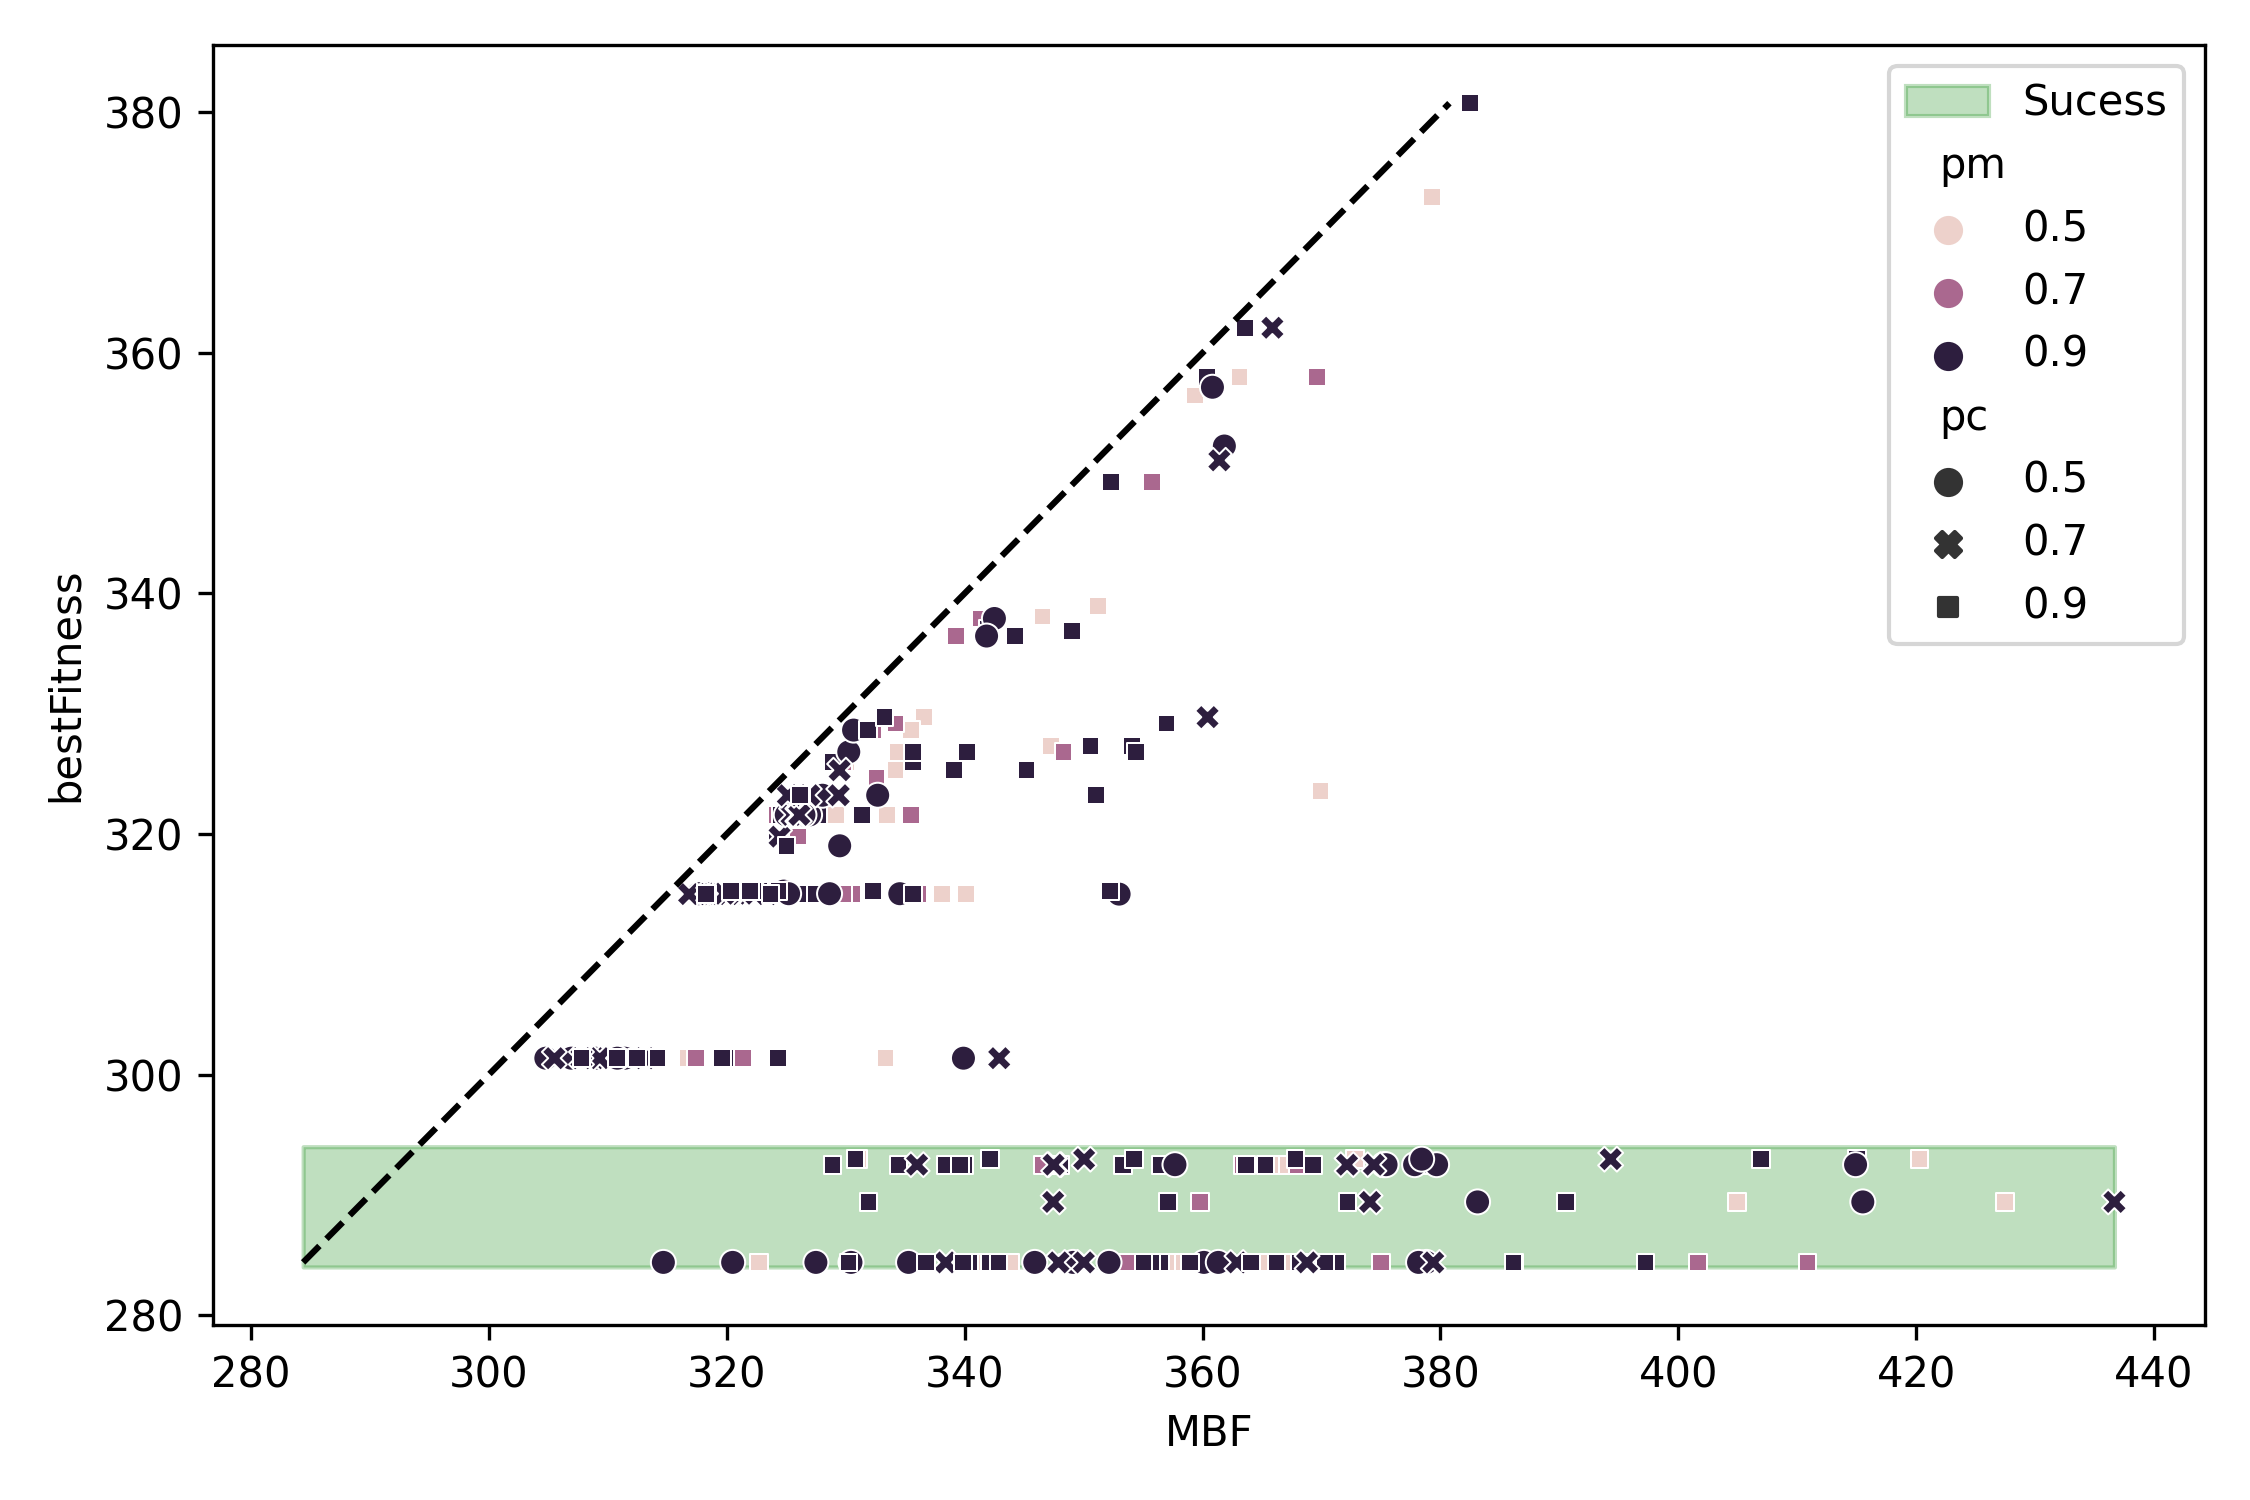
\includegraphics[scale=0.75]{../figures/16citiesMBFvsbF.png}
    \caption{Mean Best Fitness (MBF) versus best fitness value for different parameters configuration.}
    \label{fig:mbfvsbf16}
\end{figure}

A typical progress plot of this problem and its solution are shown in Figure \ref{fig:problem16}. The GA finds the optimal solution before the maximum number of iterations of 3000 is reached. The MBF was around 348, which can be easily checked by looking at the progress plot in Figure \ref{fig:progress16}. The flat progress that we can find in the plot between iterations could correspond to a local minimum. In fact, looking at Figure \ref{fig:mbfvsbf16} there are some best fitness values that appears multiple times for different values of MBF. In such cases, we can safely say that the algorithm reached a local minimum, where the different MBF could be explained by different population initializations.

\begin{figure}[h!]
    \centering
    \begin{subfigure}[b]{0.45\textwidth}
        \centering
        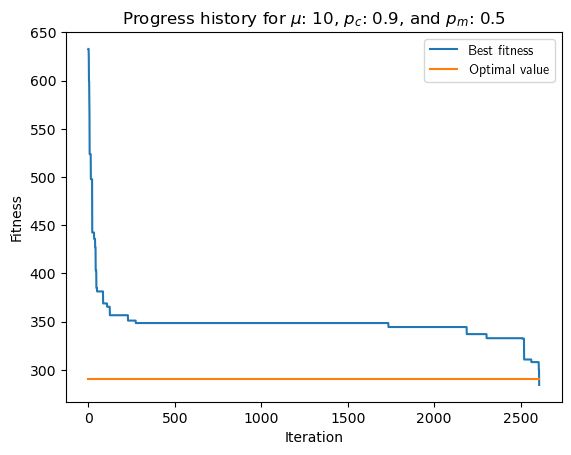
\includegraphics[width=\textwidth]{../figures/progress16.png}
        \caption{Progress for maximum number of iterations set at 3000.}
        \label{fig:progress16}
    \end{subfigure}
    \hfil
    \begin{subfigure}[b]{0.45\textwidth}
        \centering
        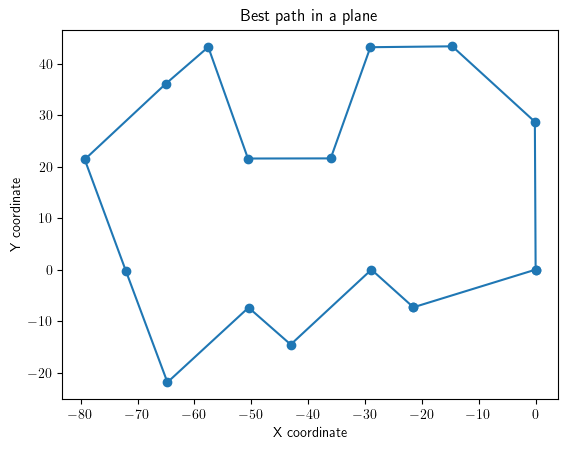
\includegraphics[width=\textwidth]{../figures/output16.png}
        \caption{Algorithm output (optimal solution)}
        \label{fig:output16}
    \end{subfigure}
    \caption{Simple problem with 16 cities reaching optimum solution}
    \label{fig:problem16}
\end{figure}

Once we fix the mutation rate to 0.9, we can individually study the importance of crossover rate in our problem. If we analyze those data points that lie into the success region we have\footnote{The SR is the count showed in Table \ref{tab:results16} divided by the total number of execution which is 50 in our case.}
\begin{table}[h!]
    \centering
    \begin{tabular}{|c|ccc|}
        \hline
        $p_c$ & 0.5 & 0.7 & 0.9 \\
        \hline
        \hline
        Count & 21 & 16 & 21 \\
        \hline
    \end{tabular}
    \caption{Single problem results for $p_m$ fixed at 0.9}
    \label{tab:results16}
\end{table}
\newpage
The results in Table \ref{tab:results16} show better performance for crossover rates of 0.5 and 0.9. On the other hand, the number of iteration required to reach the optimal value is 
\begin{table}[h!]
    \centering
    \begin{tabular}{|c|ccc|}
        \hline
        $p_c$ & 0.5 & 0.7 & 0.9 \\
        \hline
        \hline
        mean & 502.19 & 500.31 & 850.00 \\
        \hline
        std & 536.91 & 551.86 & 869.14 \\
        \hline
        min & 84 & 70 & 179 \\
        \hline 
        25 \% & 211.0 & 167.5 & 330.0 \\
        \hline
        50 \% & 287 & 253 & 435 \\
        \hline
        75 \% & 507.0 & 496.5 & 826 \\
        \hline
        max & 1923 & 1907 & 2855 \\
        \hline
    \end{tabular}
    \caption{Single problem results for $p_m$ fixed at 0.9}
    \label{tab:iters16}
\end{table}

Table \ref{tab:iters16} shows the highest efficiency for crossover rate of 0.7, i.e., the algorithm reached the solution with higher speed. Nevertheless, as we saw in Table \ref{tab:results16}, crossover rate equals to 0.7 implies lower success rate. The parameters' configuration will therefore depend on the goal and scope of our algorithm. If we would like to reach a good solution at least once, crossover rate set at 0.7 will reach the solution faster. If we would like to guarantee a better solution quality many times, crossover rates 0.5 and 0.9 increase this. In this case, we should use 0.5, since it is faster a have similar solution quality as shown in Figure \ref{fig:quality16}. Furthermore, it is worth noting that the difference between expected values of 0.5 and 0.7 could be neglected, making the final decision of parameters' configuration easier.

\begin{figure}[h!]
    \centering
    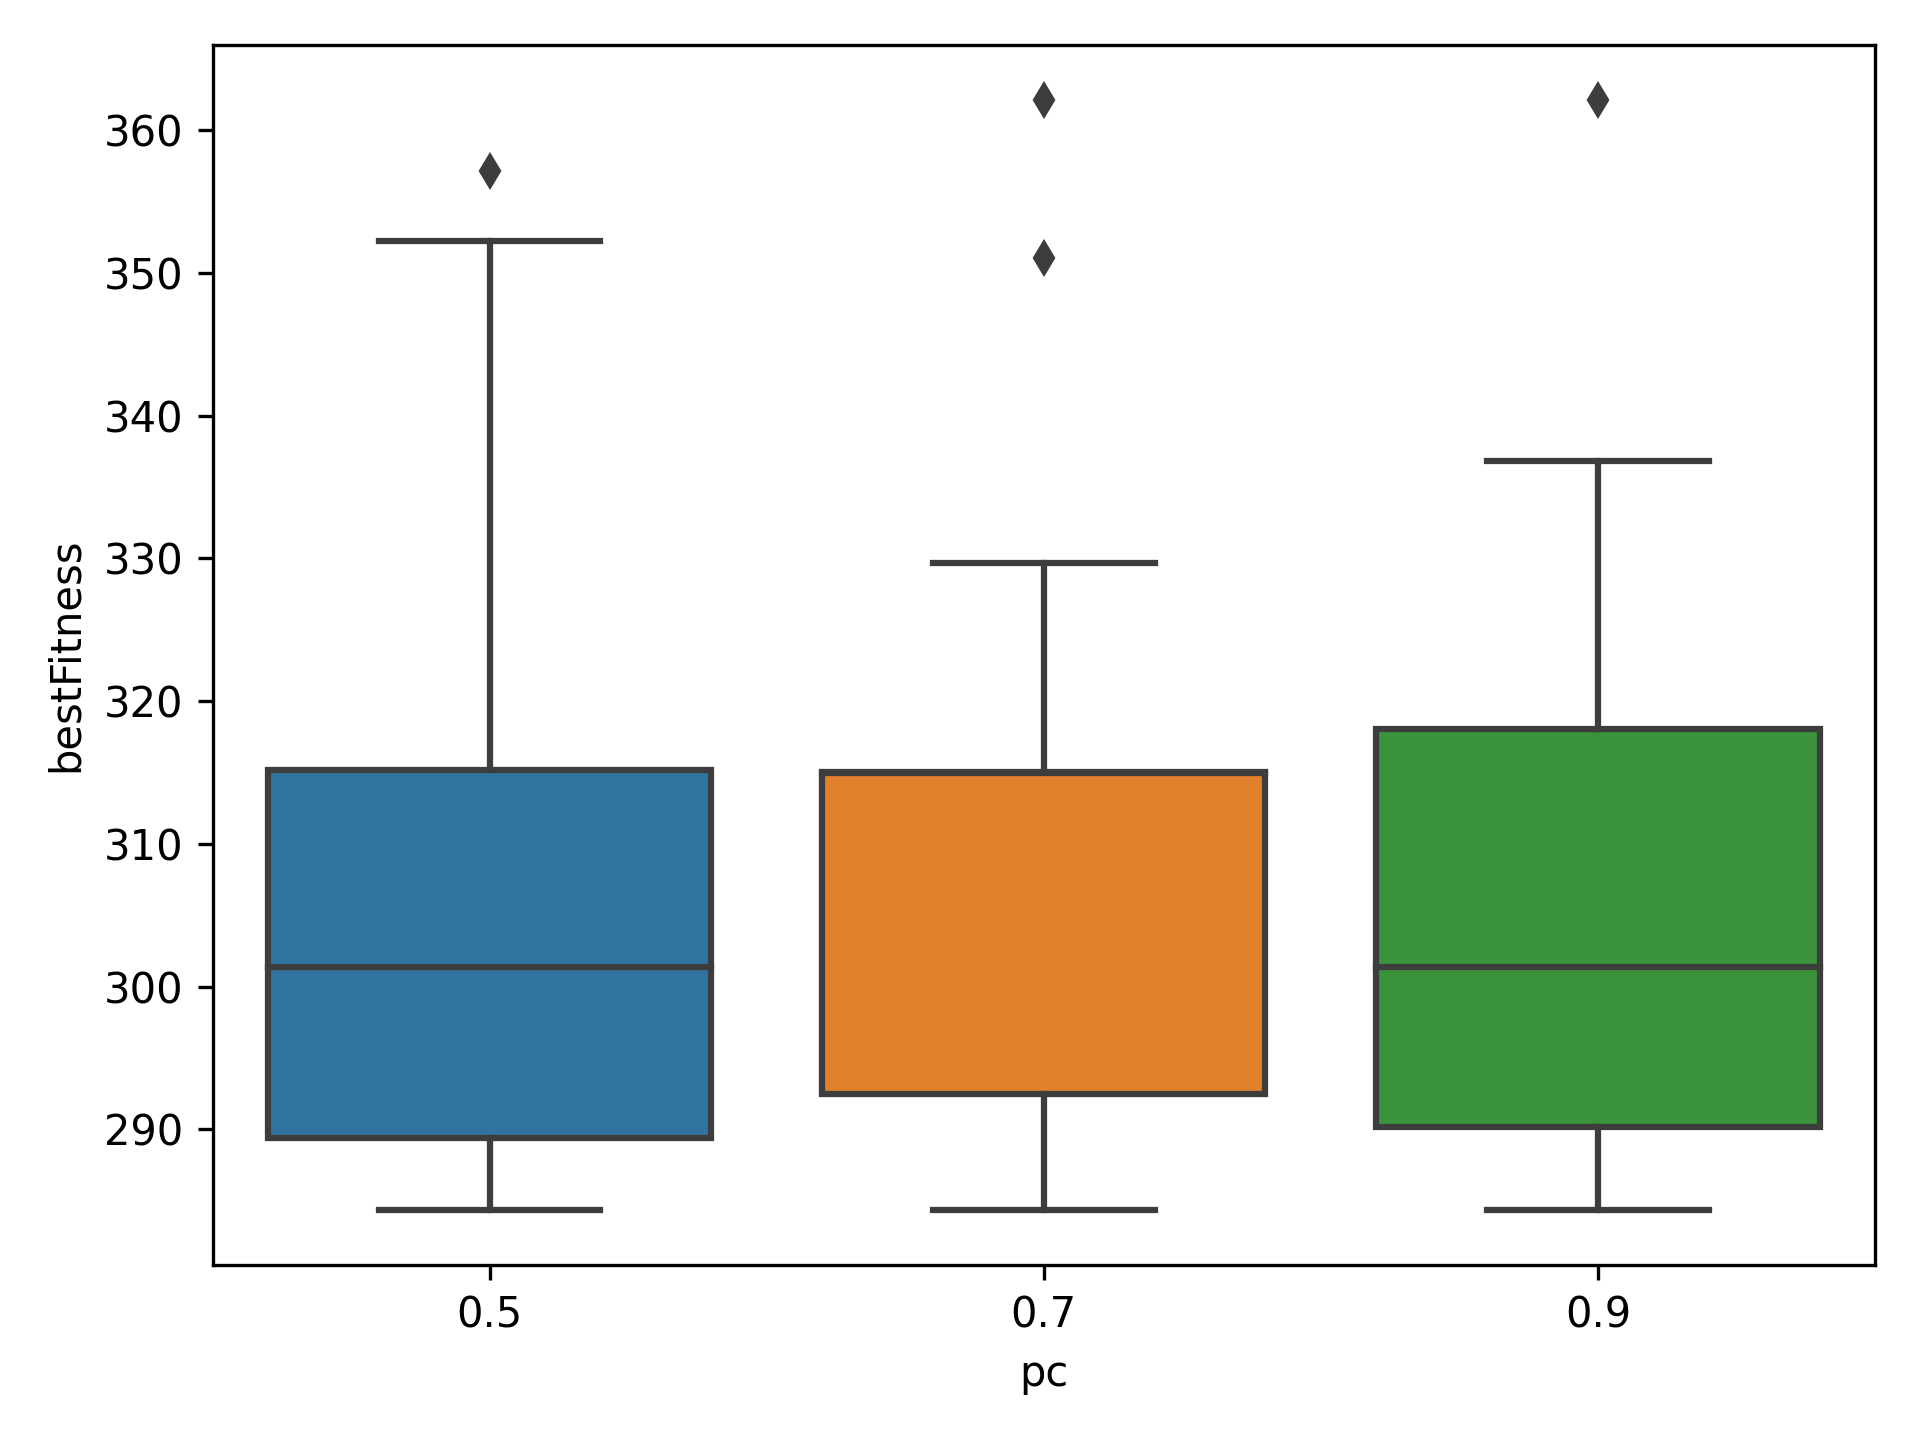
\includegraphics[scale=0.75]{../figures/16citiesquality.png}
    \caption{Solutions quality in terms of the best fitness values.}
    \label{fig:quality16}
\end{figure}

Finally, the complex problem is shown in Figure \ref{fig:mbfvsbf48}. The population size is set to 100 because of the increase in solutions space complexity. The mutation rate is also set at 0.9 without further study because of computational limitations, i.e., we just took the best value from the simple problem. Since the optimal value of 33523 is not reached at any time, we should interpret the results in a different way. Here we focus on solutions quality, meaning a lower best fitness value; and the efficiency. 

Solutions quality is studied under the boxplot showed in Figure \ref{fig:quality48}, where crossover rate of 0.9 show clearly a better performance. On the other hand, MBF and best fitness shows a linear dependency in most of the instances, meaning a similar efficiency. Indeed, once the local optima is found the best fitness get stuck on it, and only find another local optima if the variation operators are relevant enough to skip the local optima.

\newpage
\begin{figure}[h!]
    \centering
    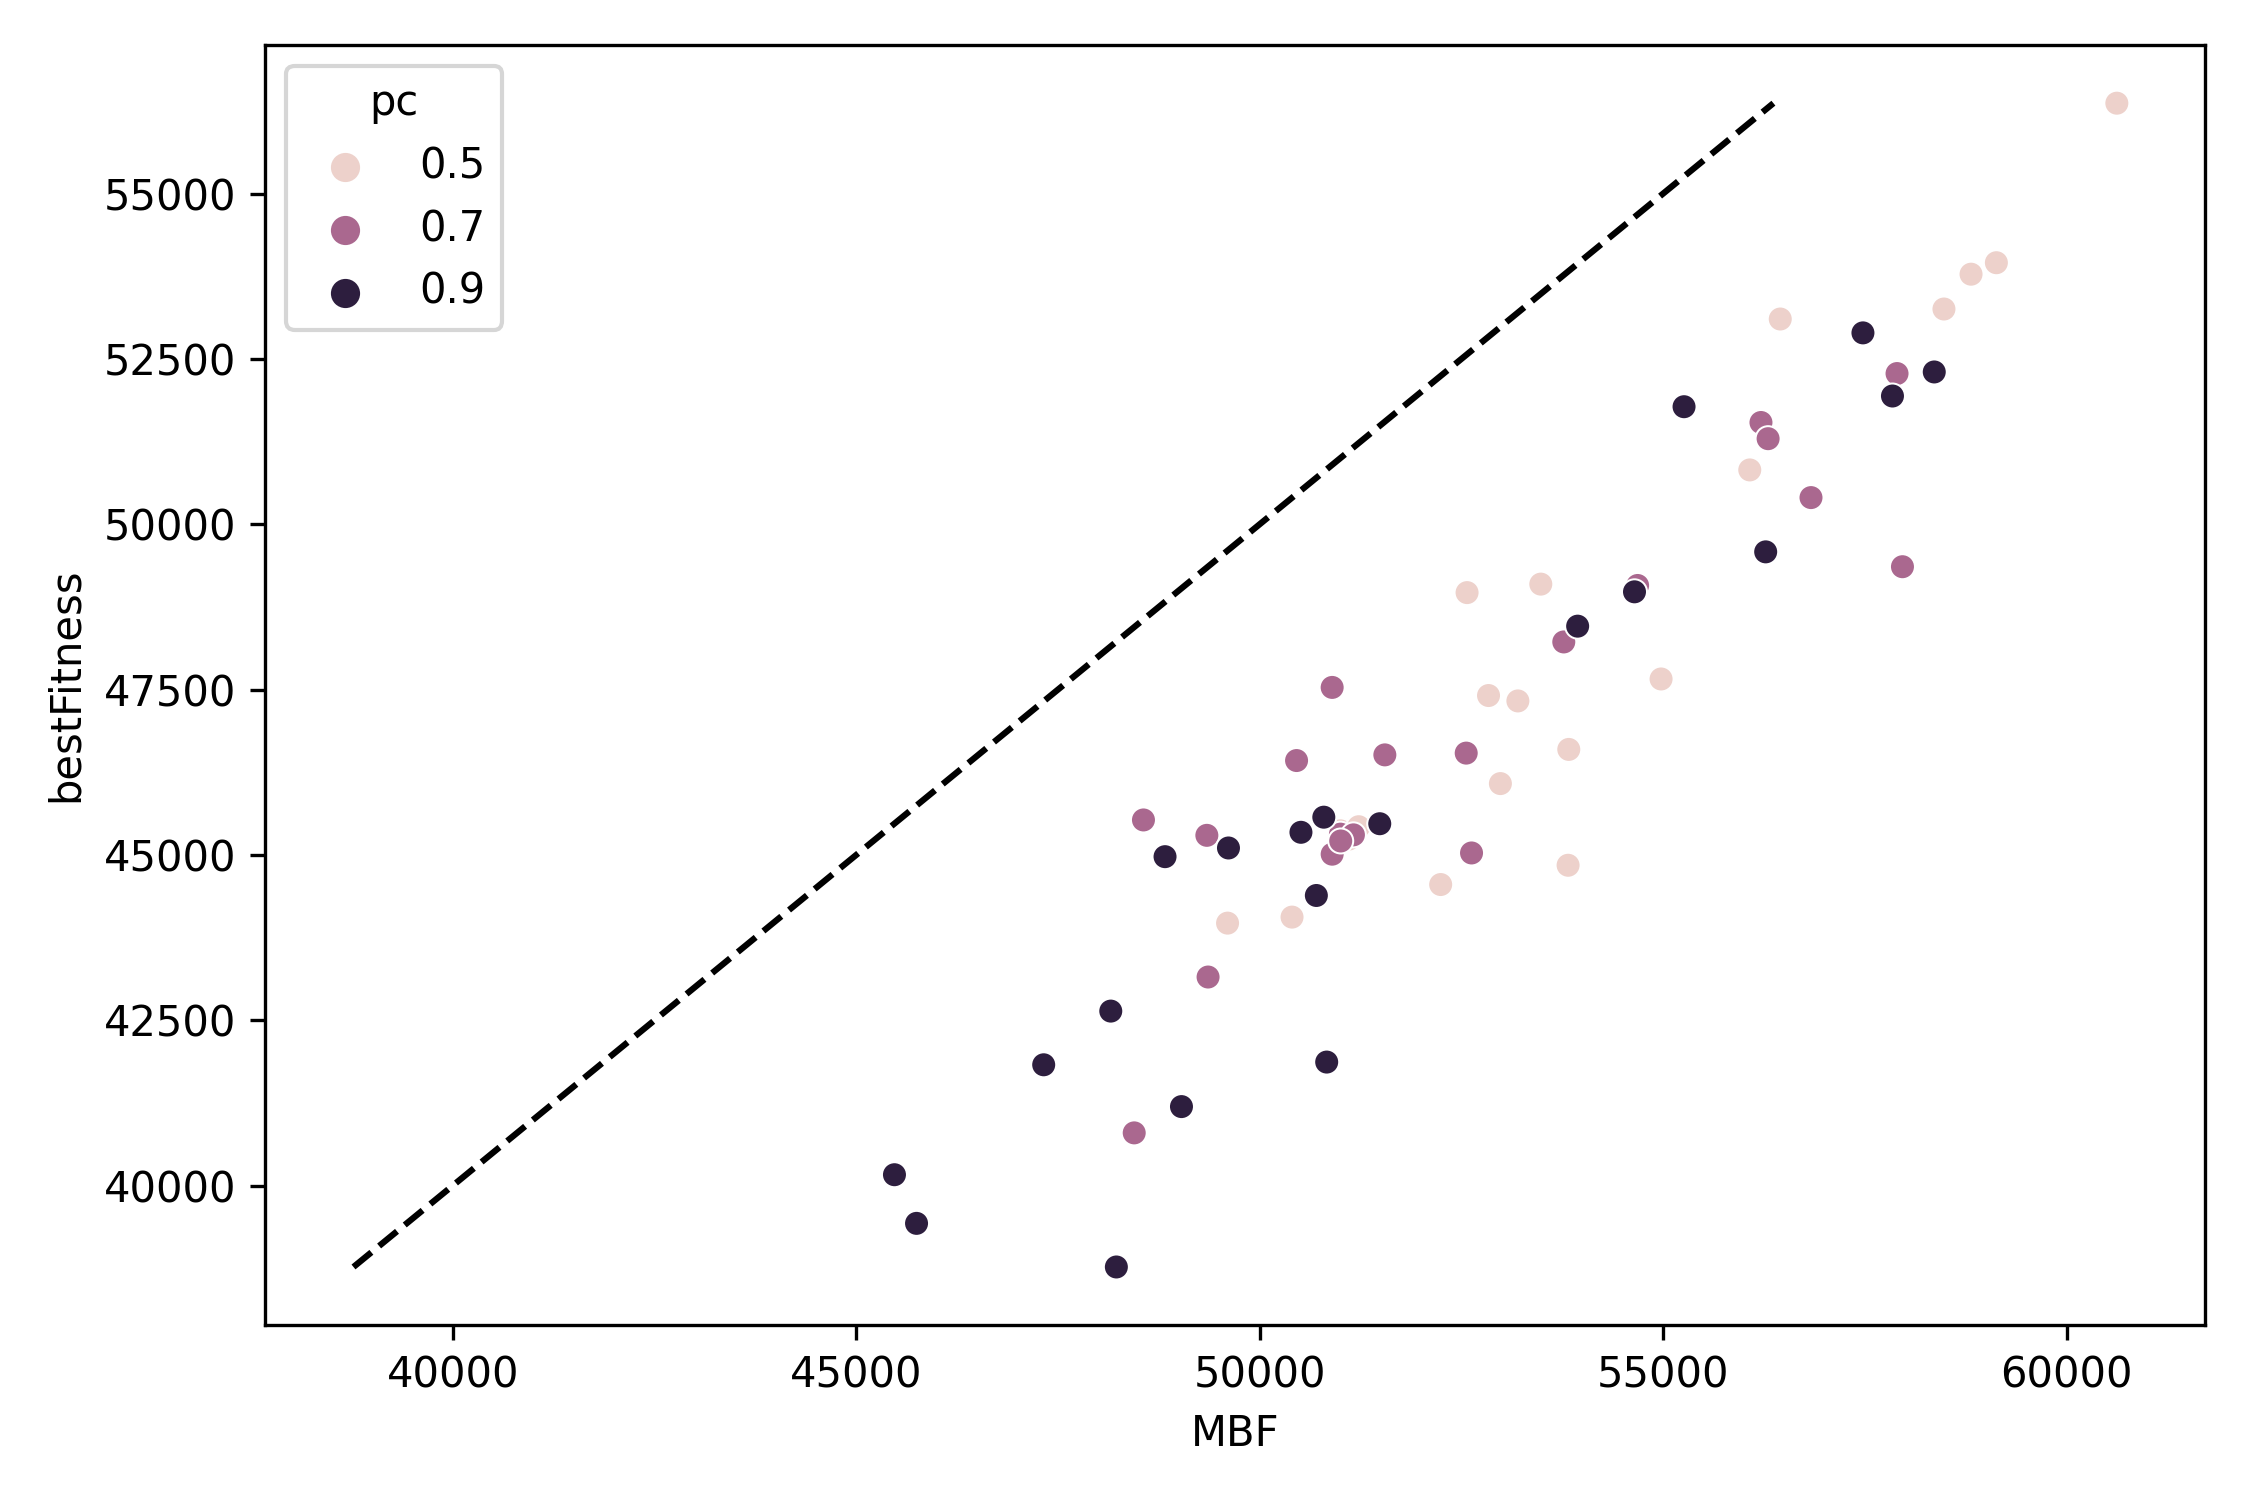
\includegraphics[scale=0.75]{../figures/48citiesMBFvsbF.png}
    \caption{Mean Best Fitness (MBF) versus best fitness value for different parameters' configuration.}
    \label{fig:mbfvsbf48}
\end{figure}

\begin{figure}[h!]
    \centering
    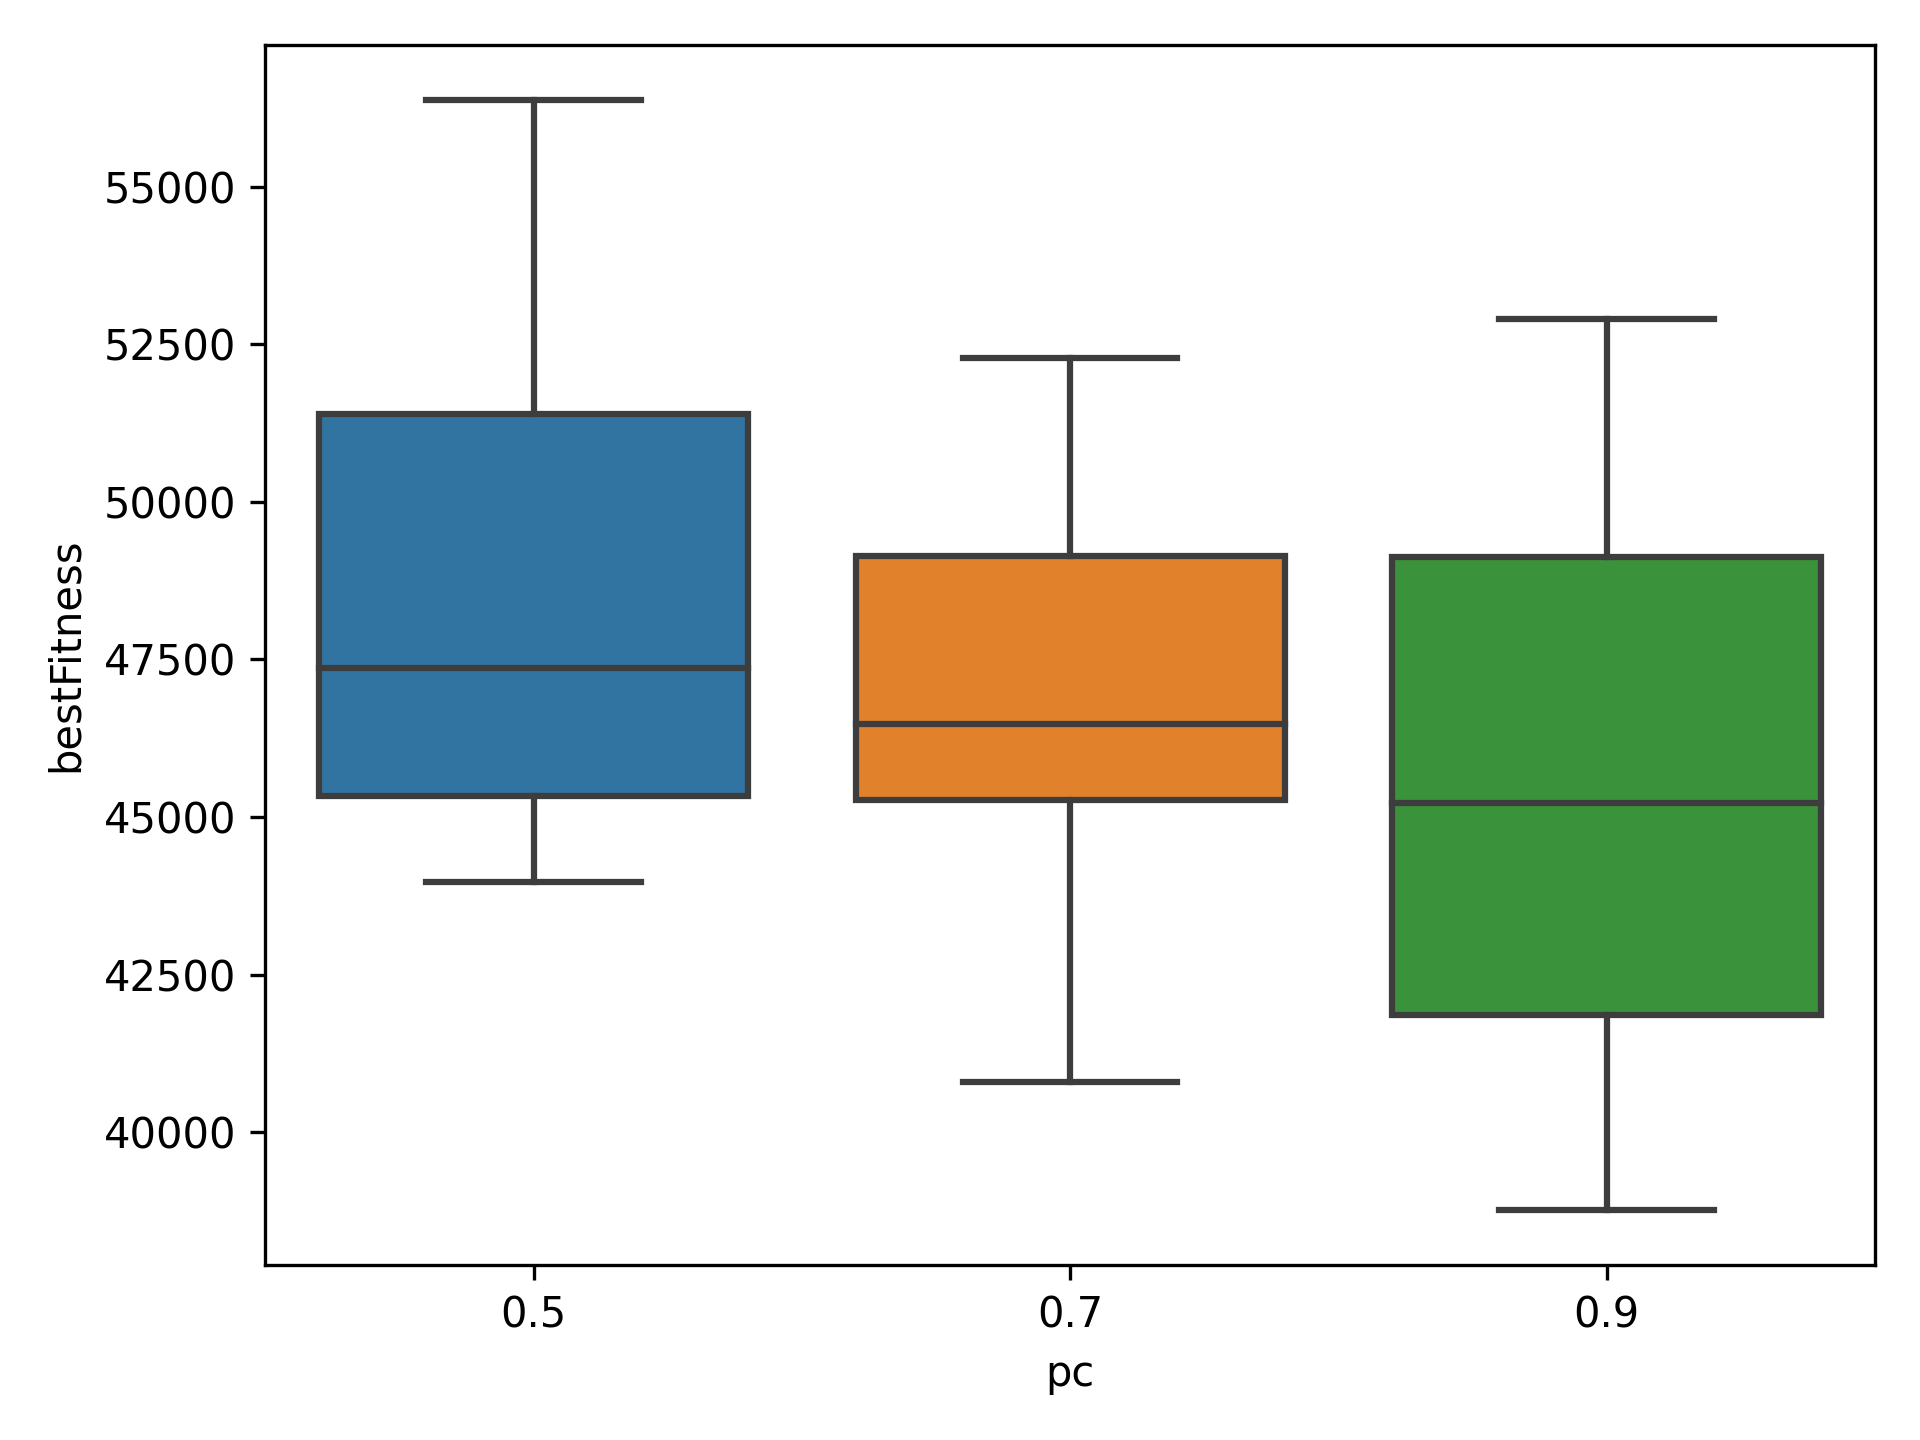
\includegraphics[scale=0.75]{../figures/48citiesquality.png}
    \caption{Solutions quality in terms of the best fitness values.}
    \label{fig:quality48}
\end{figure}

\subsection*{Synthetic datasets}
The analysis for synthetic datasets follow the same methodology as the previous examples for real-world data set, nevertheless the optimal solution is now unknown. The analysis are repeated for two problem instances of different complexity where the points (cities) are randomly drawn from a 2-dimensional uniform distribution within a given range. The solutions can be found in the Jupyter notebook.


\section{Conclusions}
The crossover rate in a genetic algorithm plays a pivotal role in balancing exploration and exploitation within the search space. A high crossover rate promotes exploration by encouraging the recombination of genetic information, potentially generating diverse offspring, which can be beneficial for escaping local optima. Conversely, a low crossover rate favors exploitation by maintaining the genetic integrity of parents, allowing for the preservation of well-performing solutions. The optimal crossover rate depends on the specific problem and its characteristics; hence, its relevance lies in its ability to fine-tune the algorithm's ability to strike a balance between exploration and exploitation, ultimately influencing the algorithm's convergence speed and solution quality.

\section*{Supplementary figures}
\begin{figure}[h!]
    \centering
    \begin{subfigure}[b]{0.45\textwidth}
        \centering
        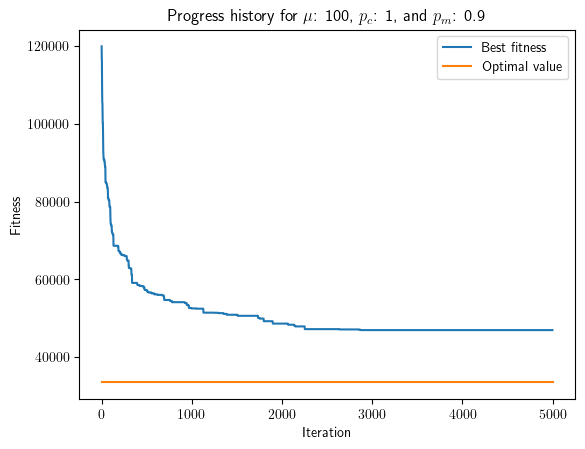
\includegraphics[width=\textwidth]{../figures/48output.png}
        \caption{Progress for maximum number of iterations set at 5000.}
        \label{fig:progress16}
    \end{subfigure}
    \hfil
    \begin{subfigure}[b]{0.45\textwidth}
        \centering
        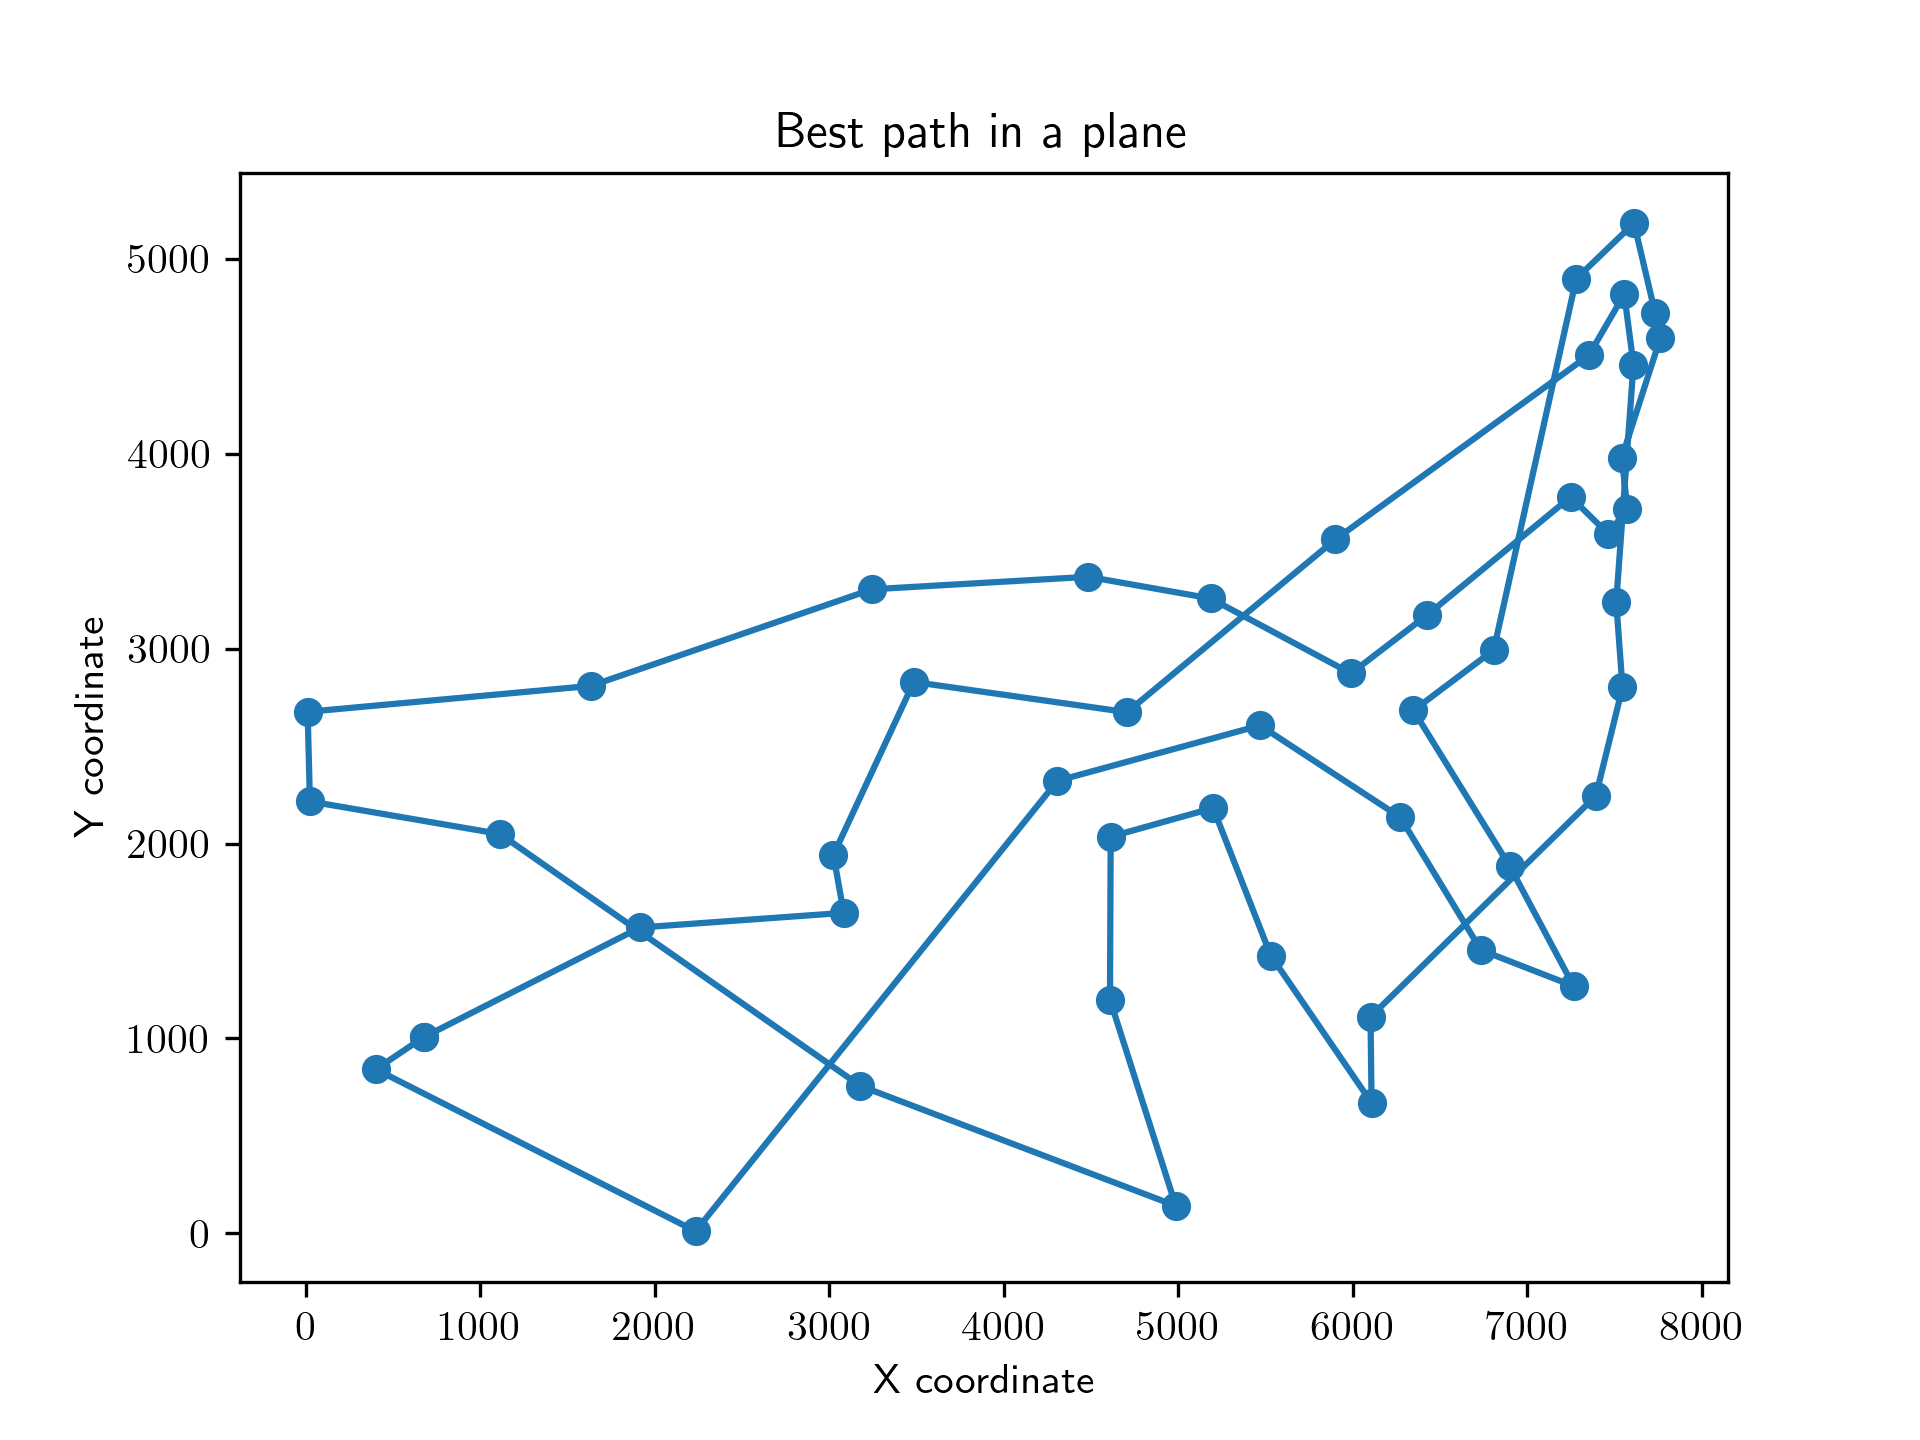
\includegraphics[width=\textwidth]{../figures/48path1.png}
        \caption{Algorithm output (local optima)}
        \label{fig:output16}
    \end{subfigure}
    \caption{Simple problem with 48 cities reaching local optima}
    \label{fig:problem16}
\end{figure}
\printbibliography

\end{document}